\noindent
% ==========================================
% CỘT TRÁI (BÀI TẬP 51, 52, 53)
% ==========================================
\begin{minipage}[t]{0.482\textwidth}

\textbf{51.} Phác thảo đồ thị của một hàm số $f$ thỏa mãn tất cả các điều kiện sau:
\begin{list}{}{\leftmargin=1.2em \itemsep=2.5pt \topsep=3pt \parsep=0pt}
    \item Tập xác định của $f$ là tất cả các số thực khác 0,
    \item $\displaystyle \lim_{x \to 0^-} f(x) = 1, \quad \lim_{x \to 0^+} f(x) = 0$,
    \item $f'(x) > 0$ với mọi $x$ thuộc tập xác định của $f$,
    \item $\displaystyle \lim_{x \to -\infty} f'(x) = 0, \quad \lim_{x \to \infty} f'(x) = 1$
\end{list}

\vspace{10pt}

\textbf{52.} Gọi $P(t)$ là tỷ lệ phần trăm người Mỹ dưới 18 tuổi tại thời điểm $t$. Bảng dưới đây cho các giá trị của hàm số này trong các năm điều tra dân số từ 1950 đến 2010.

\begin{center}
\small
\renewcommand{\arraystretch}{1.15}
\setlength{\tabcolsep}{8pt}
\begin{tabular}{|c|c||c|c|}
\hline
\rowcolor{tableheader}
$t$ & $P(t)$ & $t$ & $P(t)$ \\
\hline
1950 & 31{,}1 & 1990 & 25{,}7 \\
1960 & 35{,}7 & 2000 & 25{,}7 \\
1970 & 34{,}0 & 2010 & 24{,}0 \\
1980 & 28{,}0 &      &        \\
\hline
\end{tabular}
\end{center}

\begin{enumerate}[label=\textbf{(\alph*)}, leftmargin=*, itemsep=2pt, topsep=1pt]
    \item Ý nghĩa của $P'(t)$ là gì? Đơn vị của nó là gì?
    \item Lập bảng các giá trị ước tính cho $P'(t)$.
    \item Vẽ đồ thị của $P$ và $P'$.
    \item Làm thế nào để có thể thu được các giá trị chính xác hơn cho $P'(t)$?
\end{enumerate}

\vspace{10pt}

\textbf{53.} Gọi $B(t)$ là số lượng tờ tiền 20 đô la Mỹ đang lưu hành tại thời điểm $t$. Bảng dưới đây cho các giá trị của hàm số này từ năm 1995 đến năm 2015, tính đến ngày 31 tháng 12, theo đơn vị tỷ tờ. Hãy giải thích ý nghĩa và ước tính giá trị của $B'(2010)$.

\begin{center}
\small
\renewcommand{\arraystretch}{1.2}
\setlength{\tabcolsep}{6pt}
\begin{tabular}{|>{\columncolor{tableheader}}c|c|c|c|c|c|}
\hline
$t$ & 1995 & 2000 & 2005 & 2010 & 2015 \\
\hline
$B(t)$ & 4{,}21 & 4{,}93 & 5{,}77 & 6{,}53 & 8{,}57 \\
\hline
\end{tabular}
\end{center}

\end{minipage}%
\hfill
% ==========================================
% CỘT PHẢI (BÀI TẬP 54, 55, 56)
% ==========================================
\begin{minipage}[t]{0.482\textwidth}

\textbf{54.} \emph{Tổng tỷ suất sinh} tại thời điểm $t$, ký hiệu là $F(t)$, là ước tính số con trung bình sinh ra bởi mỗi phụ nữ (với giả định rằng tỷ lệ sinh hiện tại không đổi). Đồ thị về tổng tỷ suất sinh ở Hoa Kỳ cho thấy những biến động từ năm 1940 đến năm 2010.
\begin{enumerate}[label=\textbf{(\alph*)}, leftmargin=*, itemsep=2pt, topsep=2pt]
    \item Ước tính các giá trị của $F'(1950)$, $F'(1965)$ và $F'(1987)$.
    \item Ý nghĩa của các đạo hàm này là gì?
    \item Bạn có thể đưa ra các lý do giải thích cho giá trị của các đạo hàm này không?
\end{enumerate}

\begin{center}
    \vspace{1pt}
    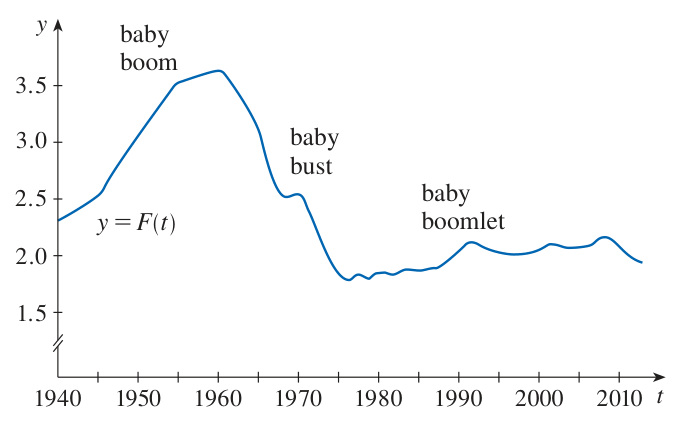
\includegraphics[width=0.92\linewidth]{images/p0205_fig1.png}
    \vspace{1pt}
\end{center}

\textbf{55.} Giả sử rằng $|f(x)| \leqslant g(x)$ với mọi $x$, trong đó $\lim_{x \to a} g(x) = 0$. Tìm $\lim_{x \to a} f(x)$.

\vspace{10pt}

\textbf{56.} Cho hàm số $f(x) = \llbracket x \rrbracket + \llbracket -x \rrbracket$.
\begin{enumerate}[label=\textbf{(\alph*)}, leftmargin=*, itemsep=2pt, topsep=2pt]
    \item Với những giá trị nào của $a$ thì $\lim_{x \to a} f(x)$ tồn tại?
    \item Hàm số $f$ gián đoạn tại những điểm nào?
\end{enumerate}

\end{minipage}
